% Provenance (never printed): see sources/outline_sources.md (Year 3: gravity, magnetic,
% seismic, resistivity and ground-penetrating-radar surveys; data processing and
% uncertainty; a mapping project).
% Brief: sources/book5/BRIEFS.md, ch. 31. Curves from figdata/bachelor-3/gravity_granite.py
% (prism model of the Varden granite of figdata/shared/region.py), magnetic_dyke.py (2-D
% dyke; the Varden dolerite dyke of the Sync 3 ruling, buried below the unconformity),
% resistivity_sounding.py (Pekeris transform and image series) and gpr_radargram.py.
% Physical-property ranges and survey practice from the GPG open textbook (CC BY 4.0) and
% Keys (1990). Exercise and problem values in the Book 5 scratch calculator calc/ch31.py.
\chapter{Field and Lab Methods III}\label{ch:b3:field-lab-methods-3}

A geophysics crew spends a week in the valley of the Varden Hills, the
invented region whose geological map the Year~1 volume drew in its
chapter on geological maps. The map shows a granite cropping out on
the sides of the valley, between the schists, under the sandstone that
rests on both. Where the granite goes under the cover, how far it
extends and how deep it reaches, no one has seen. The crew carries a
gravimeter, two magnetometers, a cable of electrodes and a radar on a
small cart. None of these instruments sees a rock: each measures a
field at the surface---gravity, the magnetic field, an electric
potential, the echo of a radio pulse---that the rocks below disturb.
By the end of the week the crew can draw the granite it never saw, say
how deep the alluvium of the valley floor is, and report a magnetic body
that no map showed.

This chapter follows that week. It treats each method in turn, as a
measurement with its corrections and as a \omterm{def:b3:seismology-imaging:inverse}{forward problem} with a few
bodies whose fields can be computed exactly; it then sets out how the
errors of a survey add up and why one kind of data rarely fixes a
model; and it ends with the Varden survey, where the methods are put
together.

\begin{recall}
The gravity anomaly, the free-air and Bouguer corrections and anomalies
and normal gravity are in the Year~1 volume, in its chapter on isostasy
and gravity; the survey loop of a \omterm{def:b3:field-lab-methods-3:gravimeter}{relative gravimeter} is described in
\cref{ch:b3:gravity-geodesy}. The main field, its inclination, the
\omterm{thm:b3:palaeomagnetism:dipole}{dipole formula} and the \omterm{def:b3:palaeomagnetism:igrf}{International Geomagnetic Reference Field} are in
\cref{ch:b3:palaeomagnetism}. Resistivity, Ohm's law, the relative
permittivity, electromagnetic waves, magnetisation and magnetic
susceptibility are in the physics books, and Gauss's theorem for
gravity with them. \omterm{def:b3:exploration-seismology:surveys}{Seismic refraction surveys} are in
\cref{ch:b3:exploration-seismology}; forward and \omterm{def:b3:seismology-imaging:inverse}{inverse problems} and
weighted least squares in \cref{ch:b3:seismology-imaging}; porosity in
the school books and \omterm{def:b3:facies-models:wireline}{wireline logs} in \cref{ch:b3:facies-models}. The
propagation of uncertainties is in the chemistry and mathematics books.
\end{recall}

\section{Gravity surveys}\label{sec:b3:field-lab-methods-3:gravity}

The anomalies that a gravity survey looks for are small. Gravity at the
equator is about \qty{978000}{\milli\gal}; large structures change it
by hundreds of milligals, a salt dome by about ten, an ore body by
about one, and the targets of a geotechnical survey by a few
hundredths. Geophysicists measure in
milligals, or in gravity units of \qty{0.1}{\milli\gal}; a useful survey
must resolve differences of one part in a hundred million of~$g$.
% ledger: gpg:grav-units, gpg:grav-sizes

\begin{definition}[Relative gravimeter; instrumental drift]\label{def:b3:field-lab-methods-3:gravimeter}
A \emph{relative gravimeter}\index{relative gravimeter} is an
instrument that measures differences of gravity between stations: a
mass on a spring, kept at a null position by a second, adjustable force
whose dial reading, multiplied by a calibration constant, gives gravity
in milligals up to an unknown constant. Its \emph{instrumental
drift}\index{instrumental drift} is the slow change of its reading at a
fixed station, caused by the creep of the spring, temperature and
shocks; it is measured by reading again, after a few hours, a station
already read, the \emph{base station}.
\end{definition}
% ledger: gpg:gravimeter, gpg:grav-survey

A field gravimeter covers a range of several tens of thousands of
milligals and reads, at its best, to about \qty{0.01}{\milli\gal}; the
range must be reset after transport. At that precision the height of
each station matters as much as its reading: \qty{3.3}{cm} of height
error spoil \qty{0.01}{\milli\gal}, so positions are surveyed with
satellite receivers or a level to the centimetre. The base station is
re-occupied every couple of hours. The solid-Earth tide, which can reach
\qty{0.3}{\milli\gal}, changes slowly enough over those hours to be
removed with the drift.
% ledger: gpg:gravimeter, gpg:grav-survey, gpg:grav-sizes

\begin{method}[Reducing a gravity loop]\label{met:b3:field-lab-methods-3:loop}
A loop starts and ends at a base station, read at times $t_0$ and $t_1$.
\begin{enumerate}
  \item Compute the drift rate $(r_1 - r_0)/(t_1 - t_0)$ from the two
        base readings; it includes the tide.
  \item Subtract from each reading the drift accumulated since $t_0$,
        $r - (t - t_0)(r_1 - r_0)/(t_1 - t_0)$, and subtract the base
        reading: this is gravity relative to the base.
  \item Correct for the height $\Delta h$ of the station above the base:
        add the free-air correction $\qty{0.3086}{\milli\gal.m^{-1}}
        \times\Delta h$ and subtract the Bouguer correction
        $\qty{0.1119}{\milli\gal.m^{-1}}\times\Delta h$ (density
        \qty{2670}{kg.m^{-3}}), that is, add $0.1967\,\Delta h$.
  \item For a station a distance $\Delta y$ north of the base, subtract
        the change of normal gravity, $\qty{0.811}{\milli\gal.km^{-1}}
        \times\sin 2\varphi\times\Delta y$.
  \item Add the \omterm{def:b3:field-lab-methods-3:terrain}{terrain correction} of each station.
\end{enumerate}
The result is the Bouguer anomaly relative to the base. Tying the base
to a station of known absolute gravity gives the anomaly itself.
\end{method}
% ledger: gpg:grav-survey, gpg:terrain

The Bouguer correction treats the ground between the station and the
reference level as a flat slab. In real relief this is wrong twice:
a hill that rises above the station pulls upward and lowers the
reading, and a valley that falls below it is counted in the slab as
rock that is not there.

\begin{definition}[Terrain correction]\label{def:b3:field-lab-methods-3:terrain}
The \emph{terrain correction}\index{terrain correction} of a gravity
station is the attraction that the departures of the relief from the
Bouguer slab exert on it: the hills above the level of the station, and
the valleys below it, counted with the density of the slab. Both lower
the measured gravity compared with the slab, so the correction is
always added.
\end{definition}

It was computed by hand, with a Hammer chart and tables, zone by zone
outward from the station; it is now computed from a digital elevation
model. Away from steep relief it rarely exceeds \qty{1}{\milli\gal},
but the zones close to the station are hard to get right, and the
correction is seldom known to better than \qty{0.2}{\milli\gal}.
% ledger: gpg:terrain, gpg:grav-sizes

\subsection{Anomalies of simple bodies}

The \omterm{def:b3:seismology-imaging:inverse}{forward problem} of gravity is a sum: each element of a body of
density contrast $\Delta\rho$ attracts the station by Newton's law, and
a survey measures the vertical component of the sum. A few bodies give
it in closed form.

\begin{theorem}[Sphere and horizontal cylinder]\label{thm:b3:field-lab-methods-3:sphere}
At a horizontal distance $x$ from the point above its centre, a buried
sphere of excess mass $\Delta m$ whose centre is at depth $z$ gives the
anomaly
\[
\Delta g(x) = \frac{G\,\Delta m\,z}{(x^2 + z^2)^{3/2}} ,
\]
and the anomaly falls to half its peak at $x_{1/2} = z\sqrt{2^{2/3} - 1}$,
so that $z = 1.305\,x_{1/2}$. A long horizontal cylinder of excess mass
$\lambda$ per unit length, its axis at depth $z$, gives across its
strike
\[
\Delta g(x) = \frac{2G\lambda z}{x^2 + z^2} ,
\]
and $z = x_{1/2}$.
\end{theorem}

\begin{proof}
Outside a sphere whose density depends only on the distance from its
centre, the attraction is that of its mass placed at the centre (the
shell theorem, a consequence of Gauss's theorem). Its magnitude at the
station is $G\Delta m/(x^2 + z^2)$, and the vertical component carries
the factor $z/\sqrt{x^2 + z^2}$. Writing $\Delta g(x_{1/2}) =
\Delta g(0)/2$ gives $(1 + x_{1/2}^2/z^2)^{3/2} = 2$, hence the rule. For
the cylinder, Gauss's theorem on a coaxial cylinder of radius $r$ gives
a field $2G\lambda/r$, and the vertical component $2G\lambda z/r^2$;
half the peak is reached when $x^2 + z^2 = 2z^2$.
\end{proof}
% ledger: gpg:half-width

A body that is not a sphere still has a half-width, and the rule then
gives the depth of an equivalent sphere, not of the body. The rule is
a first guess, made before any model is fitted.

\begin{proposition}[Vertical cylinder on its axis]\label{prop:b3:field-lab-methods-3:vcyl}
A vertical cylinder of radius $a$ and density contrast $\Delta\rho$,
whose top and bottom are at depths $z_1 < z_2$ below the station,
gives on its axis
\[
\Delta g = 2\pi G\Delta\rho\left[(z_2 - z_1) + \sqrt{z_1^2 + a^2}
           - \sqrt{z_2^2 + a^2}\right] .
\]
For $a \to \infty$ it is the Bouguer slab $2\pi G\Delta\rho(z_2 - z_1)$;
for a cylinder from the surface to great depth it tends to
$2\pi G\Delta\rho\,a$.
\end{proposition}

\begin{proof}
A disc of radius $a$ and thickness $\mathrm{d}z$ at depth $z$ attracts
a point on its axis by $2\pi G\Delta\rho\,\mathrm{d}z\,(1 -
z/\sqrt{z^2 + a^2})$, the attraction of a ring integrated over the
radius. Integrating from $z_1$ to $z_2$ gives the bracket. When $a \to
\infty$ at fixed depths, $\sqrt{z_1^2 + a^2} - \sqrt{z_2^2 + a^2} =
(z_1^2 - z_2^2)/(\sqrt{z_1^2 + a^2} + \sqrt{z_2^2 + a^2}) \to 0$; when
$z_1 = 0$ and $z_2 \to \infty$, $z_2 - \sqrt{z_2^2 + a^2} \to 0$ and
the bracket tends to $a$.
\end{proof}

\begin{proposition}[Excess mass from a gravity map]\label{prop:b3:field-lab-methods-3:gauss}
Whatever the shape of a body that lies entirely below a horizontal
plane, its excess mass is
\[
\Delta m = \frac{1}{2\pi G}\iint \Delta g\,\mathrm{d}A ,
\]
the integral covering the whole plane.
\end{proposition}

\begin{proof}
For a point mass $m$ at depth $z$, with $r$ the horizontal distance,
$\iint \Delta g\,\mathrm{d}A = \int_0^\infty
Gmz\,(r^2 + z^2)^{-3/2}\,2\pi r\,\mathrm{d}r = 2\pi Gm$: half the flux
$4\pi Gm$ of Gauss's theorem crosses the plane. A body is a sum of point
masses, and the integral is linear.
\end{proof}

The theorem gives the mass, never the shape; and a map covers only part
of the plane, while the anomaly of a deep body decays slowly, so the
mass found from a map is too small unless its edges are extended by a
model.

\begin{omfigure}
\begin{tikzpicture}
\begin{axis}[axis equal image, xmin=1.5, xmax=5.5, ymin=2.6, ymax=5.7, width=0.86\linewidth,
  tick label style={font=\scriptsize}, xlabel={east (km)}, ylabel={north (km)},
  label style={font=\small}, unbounded coords=jump]
% geology of the region (figdata/shared/region.py), faded
\addplot[lith schist, draw=black!50, line width=0.2pt, even odd rule, opacity=0.45] table {figdata/out/shared-region-unit-schist.dat};
\addplot[lith granite, draw=black!50, line width=0.2pt, even odd rule, opacity=0.45] table {figdata/out/shared-region-unit-granite.dat};
\addplot[om lith={icsTriassic!35}{om sand}, draw=black!50, line width=0.2pt, even odd rule, opacity=0.45] table {figdata/out/shared-region-unit-sandstone.dat};
\addplot[om lith={icsJurassic!40}{om limestone}, draw=black!50, line width=0.2pt, even odd rule, opacity=0.45] table {figdata/out/shared-region-unit-limestone.dat};
\addplot[om lith={icsJurassic!15}{om shale}, draw=black!50, line width=0.2pt, even odd rule, opacity=0.45] table {figdata/out/shared-region-unit-shale.dat};
\addplot[lith alluvium, draw=black!50, line width=0.2pt, even odd rule, opacity=0.45] table {figdata/out/shared-region-unit-alluvium.dat};
\addplot[river] table {figdata/out/shared-region-river.dat};
% the survey (figdata/bachelor-3/gravity_granite.py, magnetic_dyke.py)
\addplot[only marks, mark=*, mark size=0.7pt, black!70] table[x=x_km, y=y_km] {figdata/out/bachelor-3-gravity_granite-stations.dat};
\addplot[omDef, very thick] table[x=x_km, y=y_km] {figdata/out/bachelor-3-gravity_granite-contours.dat};
\addplot[omThm, thick] coordinates {(1.5,4.15) (5.5,4.15)};
\addplot[omMeth, line width=2.2pt, opacity=0.8] coordinates {(1.7,4.15) (2.7,4.15)};
\addplot[omProp, dashed, thick] coordinates {(2.2,2.6) (2.2,5.7)};
\addplot[only marks, mark=star, mark size=3.5pt, omMeth!70!black, thick] coordinates {(3.5,4.0)};
\node[font=\scriptsize, fill=white, fill opacity=0.85, text opacity=1, inner sep=1pt] at (axis cs:3.5,5.12) {$-0.5$};
\node[font=\scriptsize, fill=white, fill opacity=0.85, text opacity=1, inner sep=1pt] at (axis cs:3.5,4.84) {$-1$};
\node[font=\scriptsize, fill=white, fill opacity=0.85, text opacity=1, inner sep=1pt] at (axis cs:3.5,4.58) {$-2$};
\node[font=\scriptsize, anchor=south west, fill=white, fill opacity=0.85, text opacity=1, inner sep=1pt] at (axis cs:1.55,4.17) {gravity profile};
\node[font=\scriptsize, anchor=north, fill=white, fill opacity=0.85, text opacity=1, inner sep=1pt] at (axis cs:2.2,4.08) {magnetic line};
\node[font=\scriptsize, anchor=north west, text=omProp!80!black, fill=white, fill opacity=0.85, text opacity=1, inner sep=1pt] at (axis cs:2.24,5.6) {dyke, buried};
\node[font=\scriptsize, anchor=north, fill=white, fill opacity=0.85, text opacity=1, inner sep=1pt] at (axis cs:3.5,3.92) {sounding};
\pic at (axis cs:5.15,5.3) {northarrow};
\end{axis}
\end{tikzpicture}

\par\smallskip{\small The Varden survey over the region's geological map
(faded: schist grey, granite pink, sandstone, limestone and shale of the
cover, alluvium along the river). Black dots: the gravity stations,
\qty{200}{m} apart; blue: the Bouguer anomaly of the granite model,
contoured every \qty{0.5}{\milli\gal}; red: the gravity profile; green:
the magnetic line and the electrical sounding (star) on the valley
floor; orange dashed: the dolerite dyke that the magnetic survey finds,
buried under the cover.}\label{fig:b3:field-lab-methods-3:survey}
\end{omfigure}
% ledger: gpg:densities

\subsection{The Varden granite}

The geologists' model of the granite is an elliptical body below the
unconformity, \qty{760}{m} across east--west and \qty{1120}{m}
north--south where it meets the cover, widening downward; on the
valley sides it reaches the surface. Granite is lighter than schist:
the published density ranges are \numrange{2.50}{2.81} and
\qtyrange{2.39}{2.80}{g.cm^{-3}}. The survey's model takes
\qty{2620}{kg.m^{-3}} for the granite and \qty{2750}{kg.m^{-3}} for the
schist, a contrast of \qty{-130}{kg.m^{-3}}, and stops the granite at
\qty{1500}{m} below sea level, an assumption since nothing shows its
floor. Cut into \num{5533} right prisms whose attractions have a closed
form, the model gives the anomaly of the map above: a closed low of
\qty{-2.29}{\milli\gal} over the centre of the granite, its contours
elongated north--south like the body.
% ledger: gpg:densities

\begin{omfigure}
\begin{tikzpicture}
\begin{axis}[width=0.8\linewidth, height=0.42\linewidth, xmin=1.5, xmax=5.5, ymin=-2.6, ymax=0.2,
  xlabel={east (km)}, ylabel={$\Delta g$ (\unit{\milli\gal})},
  tick label style={font=\scriptsize}, label style={font=\small},
  legend style={font=\scriptsize, at={(0.02,0.04)}, anchor=south west}]
% computed in figdata/bachelor-3/gravity_granite.py
\addplot[omDef, very thick] table[x=x_km, y=dg_mGal] {figdata/out/bachelor-3-gravity_granite-profile.dat};
\addlegendentry{granite model}
\addplot[omThm, densely dashed, thick] table[x=x_km, y=sphere] {figdata/out/bachelor-3-gravity_granite-profile.dat};
\addlegendentry{sphere of the half-width rule}
\addplot[omMeth, densely dotted, thick] table[x=x_km, y=cyl] {figdata/out/bachelor-3-gravity_granite-profile.dat};
\addlegendentry{vertical cylinder}
\addplot[black!40, forget plot] coordinates {(1.5,0) (5.5,0)};
\addplot[black!50, densely dotted, forget plot] coordinates {(1.5,-1.1464) (5.5,-1.1464)};
\node[font=\scriptsize, black!60, anchor=south east] at (axis cs:5.45,-1.14) {half the peak};
\end{axis}
\end{tikzpicture}

\par\smallskip{\small The anomaly along the gravity profile (blue), the
sphere whose depth and mass the half-width rule gives (red dashed), and
a vertical cylinder of the same area as the granite at the unconformity,
from the ground to the model's floor (green dotted). The sphere matches
the peak and the half-width by construction but not the flanks; the
cylinder, which ignores the widening of the body, falls short at the
centre.}\label{fig:b3:field-lab-methods-3:profile}
\end{omfigure}
% ledger: gpg:half-width

\section{Magnetic surveys}\label{sec:b3:field-lab-methods-3:magnetics}

The Earth's main field is about \qty{25000}{nT} at the magnetic equator
and about \qty{70000}{nT} near the magnetic poles. Rocks that hold
magnetite add their own field to it, induced by the main field in
proportion to their susceptibility, or remanent, carried from the time
they formed. A felsic igneous rock has a susceptibility below about
\num{2e-3}, a mafic one from about \num{2e-3} to \num{0.4}; on the same
scale, one per cent of magnetite by volume gives about \num{0.03}.
% ledger: gpg:mag-field, gpg:susceptibility

\begin{definition}[Total-field anomaly; diurnal correction; reduction to the pole]\label{def:b3:field-lab-methods-3:magnetic}
Let $\mathbf{F}$ be the main field at the survey and $\Delta\mathbf{B}$
the field of the magnetised rocks.
\begin{itemize}
  \item The \emph{total-field anomaly}\index{total-field anomaly} is
        the measured intensity minus that of the main field, $\Delta T =
        |\mathbf{F} + \Delta\mathbf{B}| - |\mathbf{F}|$; when
        $|\Delta\mathbf{B}| \ll |\mathbf{F}|$ it is the projection
        $\Delta\mathbf{B}\cdot\mathbf{F}/|\mathbf{F}|$.
  \item The \emph{diurnal correction}\index{diurnal correction} removes
        the variations of the field with time: a magnetometer at a fixed
        base station records the field throughout the survey, and each
        reading $T(t)$ of the moving instrument is replaced by $T(t) -
        T_\mathrm{base}(t)$.
  \item The \emph{reduction to the pole}\index{reduction to the pole}
        computes, from the measured anomaly, the anomaly the same rocks
        would give if the main field were vertical, as at a magnetic
        pole; the anomaly then sits above its source.
\end{itemize}
\end{definition}
% ledger: gpg:mag-survey, gpg:mag-processing

The variations with time come from currents in the ionosphere, about
\qty{110}{km} up. In a day they typically amount to some
\qtyrange{20}{50}{nT}, as much as the anomaly of a small target; a
magnetic storm can change the field by thousands of nanoteslas. The
base station measures the variation, on the assumption that it is the
same over the whole survey. The main field itself, or the field of
structures larger than the survey, is removed with the IGRF, a constant
or a fitted trend.
% ledger: gpg:mag-field, gpg:mag-processing

A proton-precession magnetometer measures the frequency at which proton
spins precess in the field, which is proportional to the field; it
reads to \qty{1}{nT} and needs more than a second per reading. An
optically pumped caesium magnetometer is ten to a hundred times more
sensitive, reading to \qty{0.01}{nT}. The stations must be close enough
to put at least about three readings across the half-width of the
narrowest anomaly sought, and the shallower the source, the closer they
must be.
% ledger: gpg:mag-survey

\begin{proposition}[Anomaly of a thin dyke]\label{prop:b3:field-lab-methods-3:dyke}
A vertical dyke of thickness $t$ and susceptibility $\kappa$, striking
along the magnetic meridian, its top at depth $z$ and extending far
down, magnetised by induction in a main field $F$ of inclination $I$,
gives across its strike, if $t \ll z$,
\[
\Delta T(x) = \frac{\kappa F t\sin^2 I}{2\pi}\,\frac{z}{x^2 + z^2} ,
\]
a symmetric anomaly that falls to half its peak at $x = \pm z$: the
depth to the top of the dyke is half the full width of the anomaly at
half its peak.
\end{proposition}

\begin{proof}
The dyke is two-dimensional and the main field lies in the vertical
plane of the strike. The magnetisation $\mathbf{M} = \kappa\mathbf{F}/\mu_0$
has a component along the strike, whose poles lie at the ends of the
dyke, far away, and which gives no field; and a vertical component $M
\sin I$, which places on the top face of the dyke a magnetic charge of
$-Mt\sin I$ per unit length (with $\mathbf{M}\cdot\mathbf{n}$ as the
charge density, $\mathbf{n}$ the outward normal), the bottom face being
far away. A line charge $q$ per unit length produces, by Gauss's
theorem in two dimensions, a field $q/(2\pi r)$ along the radius. At a
station at $(x, 0)$ above a top at $(0, z)$ its downward component is
$Mt\sin I\,z/(2\pi(x^2 + z^2))$, and its horizontal component is
across the strike, perpendicular to $\mathbf{F}$. Multiplying by
$\mu_0$ and projecting on $\mathbf{F}$, whose vertical component is
$\sin I$, gives $\Delta T$. The half-peak condition is $x^2 + z^2 =
2z^2$.
\end{proof}

When the dyke strikes across the meridian, the horizontal parts of the
magnetisation and of the main field both lie in the plane of the
profile, the side faces carry charges, and the anomaly becomes
asymmetric, with a low on the side of the pole. The figure below
computes it exactly for a dyke of finite width, by adding the closed
fields of its four charged faces. The \omterm{def:b3:field-lab-methods-3:magnetic}{reduction to the pole} turns such
an anomaly back into the symmetric one of a vertical field.

\begin{omfigure}
\begin{tikzpicture}
\begin{groupplot}[group style={group size=2 by 1, horizontal sep=1.5cm},
  width=0.48\linewidth, height=0.42\linewidth,
  tick label style={font=\scriptsize}, label style={font=\small}, title style={font=\small}]
\nextgroupplot[xmin=-600, xmax=600, ymin=-6, ymax=28, xlabel={distance (\unit{m})},
  ylabel={$\Delta T$ (\unit{nT})}, title={a dyke at two inclinations},
  scaled x ticks=false,
  legend style={font=\scriptsize, at={(0.98,0.98)}, anchor=north east}]
% computed in figdata/bachelor-3/magnetic_dyke.py
\addplot[omDef, very thick] table[x=x_m, y=dT_I90] {figdata/out/bachelor-3-magnetic_dyke-generic.dat};
\addlegendentry{$I = 90^\circ$}
\addplot[omThm, thick] table[x=x_m, y=dT_I60] {figdata/out/bachelor-3-magnetic_dyke-generic.dat};
\addlegendentry{$60^\circ$, E--W strike}
\addplot[omMeth, densely dashed, thick] table[x=x_m, y=dT_I60ns] {figdata/out/bachelor-3-magnetic_dyke-generic.dat};
\addlegendentry{$60^\circ$, N--S strike}
\addplot[black!40, forget plot] coordinates {(-600,0) (600,0)};
\node[font=\scriptsize, black!60, anchor=south west] at (axis cs:-590,-5.6) {south};
\node[font=\scriptsize, black!60, anchor=south east] at (axis cs:590,-5.6) {north};
\nextgroupplot[xmin=1.7, xmax=2.7, ymin=0, ymax=40, xlabel={east (km)},
  ylabel={field $- \qty{48000}{nT}$}, title={the Varden line, as read},
  legend style={font=\scriptsize, at={(0.02,0.98)}, anchor=north west}]
\addplot[omDef, thick, mark=*, mark size=1.1pt] table[x=x_km, y expr=\thisrow{T_obs}-48000] {figdata/out/bachelor-3-magnetic_dyke-line.dat};
\addlegendentry{moving instrument}
\addplot[omThm, thick, densely dashed] table[x expr=1.7+\thisrow{t_min}/40, y expr=\thisrow{T_base}-48000] {figdata/out/bachelor-3-magnetic_dyke-base.dat};
\addlegendentry{base station}
\end{groupplot}
\end{tikzpicture}

\par\smallskip{\small Left: the \omterm{def:b3:field-lab-methods-3:magnetic}{total-field anomaly} of a vertical dyke
\qty{20}{m} thick, its top \qty{100}{m} deep, susceptibility \num{0.01},
in a field of \qty{50000}{nT}; on profiles across an east--west strike
at inclinations of \ang{90} and \ang{60}, and across a north--south
strike at \ang{60}. Right: the readings along the Varden magnetic line,
one station every \qty{50}{m} and every two minutes from west to east,
and the base station at the same times (plotted at the position the
moving instrument then had): the daytime rise of the field is half the
size of the anomaly.}\label{fig:b3:field-lab-methods-3:magnetic}
\end{omfigure}
% ledger: gpg:mag-field, gpg:susceptibility

\section{Electrical methods}\label{sec:b3:field-lab-methods-3:electrical}

Resistivity ranges more widely than any other property of rocks:
unweathered igneous and metamorphic rocks lie between about
\num{1000} and \qty{100000}{\ohm\metre}, shales between about
\num{3} and \num{30}, dry gravel and sand between a few hundred and ten
thousand; fresh water lies between about \num{1.5} and
\qty{130}{\ohm\metre} and salt water below one. Pore water conducts
better than most rock-forming minerals, by its ions, so the current
flows mainly through the pores, and the porosity, the saturation and
the salinity of the water control the resistivity of a rock.
% ledger: gpg:resistivity, gpg:conduction

\begin{theorem}[Point source on a uniform ground]\label{thm:b3:field-lab-methods-3:point-source}
A current $I$ injected at a point of the surface of a uniform ground of
resistivity $\rho$ produces at a distance $r$ the potential
\[
V(r) = \frac{\rho I}{2\pi r} .
\]
With two current electrodes A~($+I$) and B~($-I$) and two potential
electrodes M and N, the potential difference measured is
\[
\Delta V_{MN} = \frac{\rho I}{2\pi}\left(\frac{1}{AM} - \frac{1}{BM}
               - \frac{1}{AN} + \frac{1}{BN}\right) .
\]
\end{theorem}

\begin{proof}
By symmetry the current flows radially and crosses each hemisphere of
radius $r$, of area $2\pi r^2$, uniformly: $j = I/(2\pi r^2)$. Ohm's law
gives the field $E = \rho j$, and $V(r) = \int_r^\infty E\,\mathrm{d}r'
= \rho I/(2\pi r)$, taking $V = 0$ far away. The potentials of the two
electrodes add.
\end{proof}

\begin{definition}[Apparent resistivity; electrode array; vertical electrical sounding; electrical resistivity tomography]\label{def:b3:field-lab-methods-3:resistivity}
\leavevmode
\begin{itemize}
  \item The \emph{apparent resistivity}\index{apparent resistivity} of a
        four-electrode measurement is $\rho_a = K\,\Delta V_{MN}/I$, with
        the geometric factor $K = 2\pi/(1/AM - 1/BM - 1/AN + 1/BN)$: the
        resistivity of the uniform ground that would give the same
        reading.
  \item An \emph{electrode array}\index{electrode array} is a rule that
        places the four electrodes: the \emph{Wenner} array puts them
        equally spaced, $a$ apart, in the order AMNB; the
        \emph{Schlumberger} array puts M and N, $2l$ apart, at the
        centre of a much longer AB, of half-length $s$; dipole--dipole,
        pole--dipole and pole--pole arrays separate the current pair
        from the potential pair or send one electrode far away.
  \item A \emph{vertical electrical sounding}\index{vertical electrical sounding}
        expands an array about a fixed centre and plots
        $\rho_a$ against the spacing on logarithmic scales: the larger
        the spacing, the deeper the current flows.
  \item \emph{Electrical resistivity tomography}\index{electrical resistivity tomography}
        plants many electrodes along a line,
        measures many four-electrode combinations, and inverts them
        together for a section of resistivity.
\end{itemize}
\end{definition}
% ledger: gpg:dc-survey

For the Wenner array the factor is $K = 2\pi a$; for the Schlumberger
array, $K = \pi(s^2 - l^2)/(2l)$, and $\rho_a \approx 2\pi s^2(-\mathrm{d}V/
\mathrm{d}r)/I$ when $l \ll s$, with $l$ about a tenth of $s$ in
practice. A Schlumberger sounding moves only A and B for most readings,
the Wenner sounding all four electrodes. The current is a reversing
square wave, on, off, reversed, off, for several seconds each, because
the ground holds natural self-potentials, of electrochemical origin,
that a steady current could not be told from. Small soundings, with
electrodes up to about \qty{100}{m} apart, need a few hundred
milliwatts; soundings a kilometre wide use transmitters of tens of
kilowatts.
% ledger: gpg:dc-survey

\begin{omfigure}
\begin{tikzpicture}[font=\small, >=stealth]
\foreach \yo/\lab/\xs in {0/Wenner/{0,2,4,6}, -2.6/Schlumberger/{0,2.7,3.3,6}} {
  \begin{scope}[yshift=\yo cm]
    \fill[black!8] (-0.6,-1.3) rectangle (6.6,0);
    \draw[thick] (-0.6,0) -- (6.6,0);
    \node[anchor=east, font=\small\bfseries] at (-0.75,-0.4) {\lab};
    \foreach \x/\n in {0/A, 6/B} {\draw[omThm, very thick] (\x,0.25) -- (\x,-0.25); \node[omThm, above] at (\x,0.25) {\n};}
    \draw[omDef!40, thin] (0,0) .. controls (1,-1.1) and (5,-1.1) .. (6,0);
    \draw[omDef!40, thin] (0,0) .. controls (0.5,-0.6) and (5.5,-0.6) .. (6,0);
    \draw[omDef!40, thin] (0,0) .. controls (1.5,-1.6) and (4.5,-1.6) .. (6,0);
  \end{scope}}
\foreach \x/\n in {2/M, 4/N} {\draw[omDef, very thick] (\x,0.25) -- (\x,-0.25); \node[omDef, above] at (\x,0.25) {\n};}
\draw[<->] (0,0.75) -- node[above, font=\scriptsize] {$a$} (2,0.75);
\draw[<->] (2,0.75) -- node[above, font=\scriptsize] {$a$} (4,0.75);
\draw[<->] (4,0.75) -- node[above, font=\scriptsize] {$a$} (6,0.75);
\begin{scope}[yshift=-2.6cm]
\foreach \x/\n in {2.7/M, 3.3/N} {\draw[omDef, very thick] (\x,0.25) -- (\x,-0.25); \node[omDef, above] at (\x,0.25) {\n};}
\draw[<->] (0,0.75) -- node[above, font=\scriptsize] {$s$} (3,0.75);
\draw[<->] (2.7,-0.45) -- node[below, font=\scriptsize] {$2l$} (3.3,-0.45);
\end{scope}
\end{tikzpicture}

\par\smallskip{\small The two sounding arrays. Current enters at A and
leaves at B (red); the potential difference is measured between M and N
(blue); the faint lines are lines of current. The Wenner array keeps
the three spacings equal; the Schlumberger array keeps MN short and
expands AB.}\label{fig:b3:field-lab-methods-3:arrays}
\end{omfigure}

Over layered ground the \omterm{def:b3:field-lab-methods-3:resistivity}{apparent resistivity} of a sounding passes from
the resistivity of the top layer, at short spacings, to that of the
bottom one, at long spacings. Its curve between the two is the \omterm{def:b3:seismology-imaging:inverse}{forward
problem} of the sounding.

\begin{proposition}[Sounding over layers]\label{prop:b3:field-lab-methods-3:layers}
Over horizontal layers of resistivities $\rho_1, \dots, \rho_n$ and
thicknesses $h_1, \dots, h_{n-1}$, the Schlumberger \omterm{def:b3:field-lab-methods-3:resistivity}{apparent
resistivity} at half-spacing $s$ is
\[
\rho_a(s) = s^2\int_0^\infty T(\lambda)\,\lambda\,J_1(\lambda s)\,\mathrm{d}\lambda ,
\]
where $J_1$ is the Bessel function of order one and the resistivity
transform $T$ is built from the bottom up, $T_n = \rho_n$ and
\[
T_i = \frac{T_{i+1} + \rho_i\tanh(\lambda h_i)}{1 + T_{i+1}\tanh(\lambda h_i)/\rho_i} ,
\qquad T = T_1 .
\]
For two layers, with $k = (\rho_2 - \rho_1)/(\rho_2 + \rho_1)$,
\[
\frac{\rho_a}{\rho_1} = 1 + 2\sum_{n=1}^{\infty} k^n
  \left[1 + \left(\frac{2nh_1}{s}\right)^2\right]^{-3/2} ,
\]
the sum of the images of the source in the interface and the surface.
\end{proposition}
The integral form is admitted; the two-layer series follows from
\cref{thm:b3:field-lab-methods-3:point-source} by the method of images,
the source being reflected again and again, with a factor $k$ each
time, in the interface and in the surface.

\begin{proposition}[A conductive cover on an insulating base]\label{prop:b3:field-lab-methods-3:conductance}
If layers of total longitudinal conductance $S = \sum_i h_i/\rho_i$ rest
on a much more resistive base, the Schlumberger \omterm{def:b3:field-lab-methods-3:resistivity}{apparent resistivity} at
spacings much larger than the cover is $\rho_a = s/S$: a straight line
of slope one on the logarithmic plot, which gives $S$ but not the
thicknesses and resistivities separately.
\end{proposition}

\begin{proof}
At large spacings the current, unable to enter the base, flows
horizontally through the cover, which behaves as a sheet of
conductance $S$. Across a cylinder of radius $r$ around one electrode
the current $I$ crosses the area $2\pi r\sum h_i$, and the horizontal
field is $E = I/(2\pi rS)$. In the Schlumberger formula $-\mathrm{d}V/
\mathrm{d}r = E$, so $\rho_a = 2\pi s^2 E/I = s/S$. Any cover with the
same $S$ gives the same branch.
\end{proof}

\begin{proposition}[Archie's law]\label{prop:b3:field-lab-methods-3:archie}
A clean rock (one free of shale) fully saturated with water of
resistivity $\rho_w$ has the resistivity
\[
\rho = a\,\rho_w\,\phi^{-m} ,
\]
where $\phi$ is its porosity, $a$ a coefficient usually close to $1$
and $m$ the cementation exponent, usually between \num{1.3} and
\num{2.8} when $a = 1$. The ratio $F = \rho/\rho_w$ is the formation
factor.
\end{proposition}
% ledger: keys:archie
This is \emph{Archie's law}\index{Archie's law}, an empirical relation
set out by Archie in 1942; it has no proof, only a range of validity. It turns a resistivity into a porosity once the water is
known, and the uncertainty of $m$ is the largest in the result.

\begin{omfigure}
\begin{tikzpicture}
\begin{groupplot}[group style={group size=2 by 1, horizontal sep=1.6cm},
  width=0.48\linewidth, height=0.46\linewidth, xmode=log, ymode=log,
  tick label style={font=\scriptsize}, label style={font=\small}, title style={font=\small}]
\nextgroupplot[xmin=0.1, xmax=100, ymin=0.08, ymax=20, xlabel={$s/h_1$},
  ylabel={$\rho_a/\rho_1$}, title={two-layer curves}]
% computed in figdata/bachelor-3/resistivity_sounding.py
\addplot[omDef, thick] table[x=s_over_h, y=k_09] {figdata/out/bachelor-3-resistivity_sounding-curves.dat};
\addplot[omDef!75, thick] table[x=s_over_h, y=k_06] {figdata/out/bachelor-3-resistivity_sounding-curves.dat};
\addplot[omDef!50, thick] table[x=s_over_h, y=k_03] {figdata/out/bachelor-3-resistivity_sounding-curves.dat};
\addplot[black!50, thick] table[x=s_over_h, y=k_0] {figdata/out/bachelor-3-resistivity_sounding-curves.dat};
\addplot[omThm!50, thick] table[x=s_over_h, y=k_m03] {figdata/out/bachelor-3-resistivity_sounding-curves.dat};
\addplot[omThm!75, thick] table[x=s_over_h, y=k_m06] {figdata/out/bachelor-3-resistivity_sounding-curves.dat};
\addplot[omThm, thick] table[x=s_over_h, y=k_m09] {figdata/out/bachelor-3-resistivity_sounding-curves.dat};
\node[font=\scriptsize, anchor=north east, omDef] at (axis cs:95,10) {$k = 0.9$};
\node[font=\scriptsize, anchor=south east, omThm] at (axis cs:90,0.058) {$k = -0.9$};
\nextgroupplot[xmin=1, xmax=100, ymin=200, ymax=6000, xlabel={$s = AB/2$ (\unit{m})},
  ylabel={$\rho_a$ (\unit{\ohm\metre})}, title={the Varden sounding},
  legend style={font=\scriptsize, at={(0.03,0.97)}, anchor=north west}]
\addplot[only marks, mark=*, mark size=1.4pt, black] table[x=s_m, y=rho_obs] {figdata/out/bachelor-3-resistivity_sounding-field.dat};
\addlegendentry{readings}
\addplot[omDef, thick] table[x=s_m, y=rho_model] {figdata/out/bachelor-3-resistivity_sounding-varden.dat};
\addlegendentry{three-layer model}
\addplot[omThm, densely dashed, domain=8:100, samples=2] {x/0.02275};
\addlegendentry{$s/S$}
\end{groupplot}
\end{tikzpicture}

\par\smallskip{\small Left: Schlumberger curves over two layers, for
reflection factors $k$ from \num{0.9} (resistive base, blue, top) to
\num{-0.9} (conductive base, red, bottom). Right: the sounding on the
Varden valley floor, its readings and the model that produced them (dry
alluvium over saturated alluvium over granite), with the line $\rho_a =
s/S$ of the whole alluvium.}\label{fig:b3:field-lab-methods-3:ves}
\end{omfigure}
% ledger: gpg:resistivity, keys:archie

\section{Seismic refraction and radar in the field}\label{sec:b3:field-lab-methods-3:radar}

The \omterm{def:b3:exploration-seismology:surveys}{seismic refraction survey} of \cref{ch:b3:exploration-seismology}
is the field geophysicist's other way to the depth of a layer: a line
of geophones, a weight drop as the source, and the first arrivals
plotted against the offset, whose slopes give the velocities and whose
intercepts give the depths of the refractors. Over the Varden floor it
would see the top of the granite, faster than any sediment above it; it
could not see a layer slower than the one above, the blind spot of the
method.
% ledger: mavko:velocities

\begin{definition}[Ground-penetrating radar; radargram]\label{def:b3:field-lab-methods-3:gpr}
\emph{Ground-penetrating radar}\index{ground-penetrating radar} sends
short pulses of radio waves, of frequencies from about \qty{100}{MHz}
to \qty{1}{GHz} and durations of a few nanoseconds, from an antenna on
the ground, and records the echoes from contrasts of permittivity and
conductivity below. A \emph{radargram}\index{radargram} is the display
of the recorded traces side by side along the profile, the two-way
travel time increasing downward.
\end{definition}
% ledger: gpg:gpr

\begin{proposition}[Radar velocity, reflection and penetration]\label{prop:b3:field-lab-methods-3:radar}
In a non-magnetic ground whose conductivity $\sigma$ is small compared
with $\omega\varepsilon$, the radar pulse travels at
\[
V = \frac{c}{\sqrt{\varepsilon_r}} ,
\]
an interface between relative permittivities $\varepsilon_1$ and
$\varepsilon_2$ reflects at normal incidence the fraction $R =
(\sqrt{\varepsilon_1} - \sqrt{\varepsilon_2})/(\sqrt{\varepsilon_1} +
\sqrt{\varepsilon_2})$ of the amplitude, and the amplitude falls by a
factor $\mathrm{e}$ over the skin depth
\[
\delta = \frac{2}{\sigma}\sqrt{\frac{\varepsilon_0\varepsilon_r}{\mu_0}}
       \approx \qty{0.0053}{S}\times\frac{\sqrt{\varepsilon_r}}{\sigma} .
\]
\end{proposition}
% ledger: gpg:gpr-skin

\begin{proof}
The speed of an electromagnetic wave in a medium of permittivity
$\varepsilon_0\varepsilon_r$ and permeability $\mu_0$ is
$1/\sqrt{\mu_0\varepsilon_0\varepsilon_r}$. The reflection coefficient
is that of two media of refractive indices $\sqrt{\varepsilon_1}$ and
$\sqrt{\varepsilon_2}$. A small conductivity gives the wave number an
imaginary part $\alpha = (\sigma/2)\sqrt{\mu_0/(\varepsilon_0
\varepsilon_r)}$, whose inverse is $\delta$; with $\sqrt{\varepsilon_0/
\mu_0} = 1/(\qty{376.7}{\ohm})$ the factor is \qty{0.0053}{S}.
\end{proof}

Velocities run from \qty{0.3}{m.ns^{-1}} in air to about \num{0.15} in
dry sand, \num{0.13} in granite and \num{0.06} in saturated sand or
clay, where the permittivity of the water dominates. The useful depth
is about three skin depths: in a limestone of permittivity~6 and
conductivity \qty{1}{mS.m^{-1}} the skin depth is about \qty{13}{m},
in a clay of permittivity~20 and \qty{10}{mS.m^{-1}} about
\qty{2.4}{m}. A layer is seen if it is at least a quarter of a
wavelength thick, so higher frequencies give sharper pictures of
shallower ground.
% ledger: gpg:gpr-table, gpg:gpr, gpg:gpr-skin

\begin{proposition}[Diffraction hyperbola]\label{prop:b3:field-lab-methods-3:hyperbola}
An antenna moved along the surface above a small buried object at
$(x_p, d)$, in ground of velocity $V$, records its echo at the two-way
time
\[
t(x) = \frac{2}{V}\sqrt{(x - x_p)^2 + d^2} ,
\]
a hyperbola with apex $t_0 = 2d/V$ over the object. Any other point
$(x, t)$ of it gives $V = 2|x - x_p|/\sqrt{t^2 - t_0^2}$, and then $d =
Vt_0/2$.
\end{proposition}

\begin{proof}
The echo travels to the object and back along the straight slant path,
of length $\sqrt{(x - x_p)^2 + d^2}$ each way; squaring $t$ and
subtracting $t_0^2$ gives $V$.
\end{proof}
% ledger: gpg:gpr

\begin{omfigure}
\begin{tikzpicture}
\begin{groupplot}[group style={group size=2 by 1, horizontal sep=1.5cm},
  width=0.48\linewidth, height=0.42\linewidth,
  tick label style={font=\scriptsize}, label style={font=\small}, title style={font=\small}]
\nextgroupplot[xmin=0, xmax=8, ymin=-2.2, ymax=0.6, xlabel={distance (\unit{m})},
  ylabel={elevation (\unit{m})}, title={the ground}, axis equal image=false]
\fill[black!6] (axis cs:0,-1.5) rectangle (axis cs:8,0);
\fill[omDef!15] (axis cs:0,-2.2) rectangle (axis cs:8,-1.5);
\draw[thick] (axis cs:0,0) -- (axis cs:8,0);
\draw[omDef, thick] (axis cs:0,-1.5) -- (axis cs:8,-1.5);
\fill[black] (axis cs:4,-0.8) circle[radius=2.2pt];
\draw[omThm!70, thin, ->] (axis cs:1.5,0) -- (axis cs:4,-0.75);
\draw[omThm!70, thin, ->] (axis cs:2.5,0) -- (axis cs:4,-0.75);
\draw[omThm!70, thin, ->] (axis cs:3.5,0) -- (axis cs:4,-0.75);
\draw[omThm!70, thin, ->] (axis cs:4,0) -- (axis cs:4,-0.75);
\draw[omThm!70, thin, ->] (axis cs:4.5,0) -- (axis cs:4,-0.75);
\draw[omThm!70, thin, ->] (axis cs:5.5,0) -- (axis cs:4,-0.75);
\draw[omThm!70, thin, ->] (axis cs:6.5,0) -- (axis cs:4,-0.75);
\fill[omThm] (axis cs:1.41,0.08) rectangle (axis cs:1.59,0.2);
\fill[omThm] (axis cs:2.41,0.08) rectangle (axis cs:2.59,0.2);
\fill[omThm] (axis cs:3.41,0.08) rectangle (axis cs:3.59,0.2);
\fill[omThm] (axis cs:3.91,0.08) rectangle (axis cs:4.09,0.2);
\fill[omThm] (axis cs:4.41,0.08) rectangle (axis cs:4.59,0.2);
\fill[omThm] (axis cs:5.41,0.08) rectangle (axis cs:5.59,0.2);
\fill[omThm] (axis cs:6.41,0.08) rectangle (axis cs:6.59,0.2);
\node[font=\scriptsize, anchor=west] at (axis cs:4.15,-0.85) {pipe};
\node[font=\scriptsize, anchor=north west, fill=white, inner sep=1pt] at (axis cs:0.1,-0.05) {dry alluvium};
\node[font=\scriptsize, anchor=north west] at (axis cs:0.1,-1.55) {saturated alluvium};
\node[font=\scriptsize, anchor=south east] at (axis cs:7.9,0.22) {antenna positions};
\nextgroupplot[xmin=0, xmax=8, ymin=0, ymax=30, y dir=reverse, xlabel={distance (\unit{m})},
  ylabel={two-way time (\unit{ns})}, title={the radargram}]
% computed in figdata/bachelor-3/gpr_radargram.py
\addplot[omThm, very thick] table[x=x_m, y=t_ns] {figdata/out/bachelor-3-gpr_radargram-pipe.dat};
\addplot[omDef, very thick] table[x=x_m, y=t_ns] {figdata/out/bachelor-3-gpr_radargram-table.dat};
\node[font=\scriptsize, anchor=south] at (axis cs:4,10.2) {apex};
\node[font=\scriptsize, anchor=north west, omDef] at (axis cs:0.1,20.6) {water table};
\end{groupplot}
\end{tikzpicture}

\par\smallskip{\small A radar profile over the alluvial floor: a drain
pipe \qty{0.8}{m} deep and the water table \qty{1.5}{m} deep in alluvium
of relative permittivity~4 (left), and the arrival times of their
echoes (right). The pipe returns a hyperbola, whose flanks the antenna
records before it is above the pipe; the water table, a plane, returns a
flat echo.}\label{fig:b3:field-lab-methods-3:radargram}
\end{omfigure}
% ledger: gpg:gpr-table

\section{Processing and uncertainty}\label{sec:b3:field-lab-methods-3:processing}

Every number in a survey carries an error, and the reduction adds the
errors of the corrections to that of the reading. When the errors are
independent, their variances add.

\begin{method}[An error budget]\label{met:b3:field-lab-methods-3:budget}
\begin{enumerate}
  \item List the independent sources of error of the reduced value: the
        reading, the position and height, the density or susceptibility
        assumed, the drift or diurnal model, the terrain.
  \item Convert each into the unit of the result, multiplying by the
        derivative of the reduction with respect to it.
  \item Add the squares and take the square root.
  \item Compare the total with the size of the anomaly sought: if it is
        larger, improve the largest term first.
\end{enumerate}
\end{method}

A model is judged by how well it reproduces the data, and the measure
must weigh each datum by its uncertainty.

\begin{definition}[Data misfit]\label{def:b3:field-lab-methods-3:inversion-practice}
The \emph{misfit}\index{misfit (data)} of a model to $N$ data $d_i$ of
standard deviations $\sigma_i$ is
\[
\chi^2 = \sum_{i=1}^N\left(\frac{d_i - d_i^{\,\mathrm{model}}}{\sigma_i}\right)^2 .
\]
A model that explains the data to within their errors has $\chi^2$ close
to $N$; a much larger value means the model is wrong, a much smaller one
that it fits the noise.
\end{definition}

Minimising the \omterm{def:b3:field-lab-methods-3:inversion-practice}{misfit} is the weighted least squares of
\cref{ch:b3:seismology-imaging}. The difficulty of the potential
methods is that many models reach the same \omterm{def:b3:field-lab-methods-3:inversion-practice}{misfit}. Outside a body, its
gravity is that of an infinity of others: every sphere with the same
excess mass and centre gives the same anomaly, whatever its radius and
density; a gravity map fixes the excess mass, but not the shape; a
sounding over a conductive cover fixes the conductance $S$, but not the
thicknesses; the anomaly of a thin dyke fixes the product $\kappa t$,
but not $\kappa$ and $t$ apart. An inversion chooses among the
equivalent models by adding information: a density measured on samples,
a depth from a borehole, a smoothness imposed on the model. The surest
addition is another method, sensitive to another property: gravity sees
density, magnetics magnetite, resistivity water, radar permittivity, and
each sees what the others miss.

\section{A mapping project}\label{sec:b3:field-lab-methods-3:project}

\begin{inthefield}[A week in the valley]
\begin{minipage}[t]{0.55\linewidth}\vspace{0pt}
The crew of the Varden survey divides its week among the methods. One
member carries the gravimeter round a grid of stations \qty{200}{m}
apart, levelling it at each, while a colleague surveys the heights with
a satellite receiver; every two hours they return to the base station
by the bridge. A magnetometer is left at a base station away from the
power line and the road, recording all day, while a second is walked
along the lines. On the valley floor two others lay out the cable,
push the steel electrodes into the alluvium and expand a sounding from
a few metres to two hundred; a small radar on a cart is pulled along
the floor. In the evening the readings are reduced, and the next day's
lines are chosen from the maps of the day before.
\end{minipage}\hfill
\begin{minipage}[t]{0.42\linewidth}\vspace{0pt}
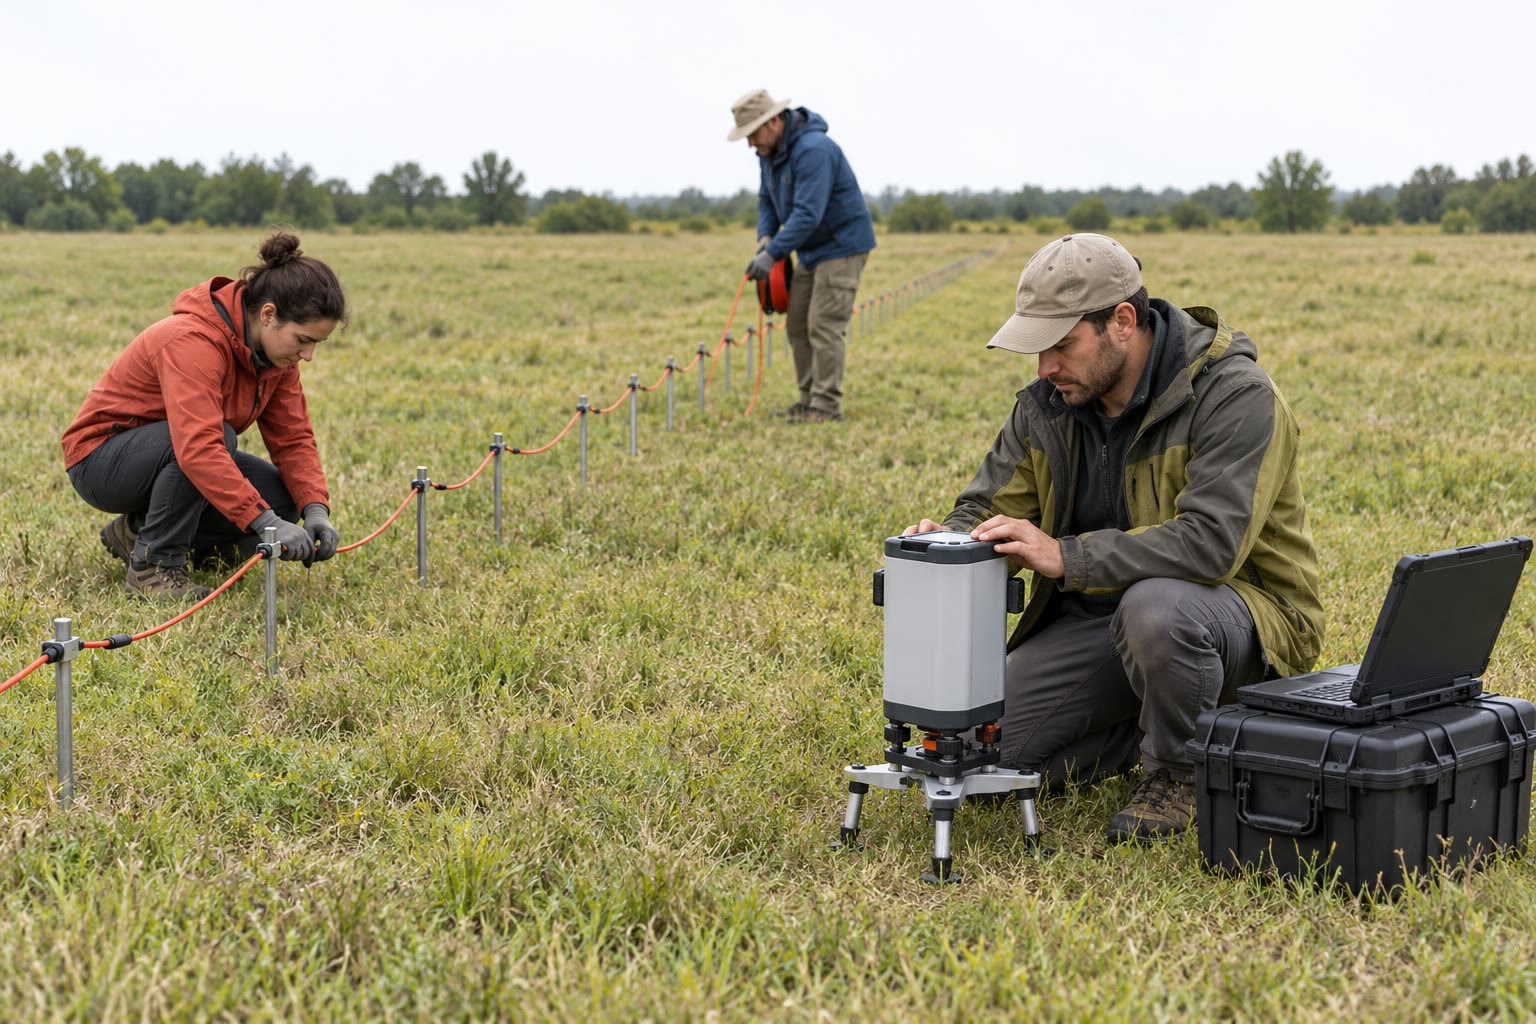
\includegraphics[width=\linewidth]{images/book5/ai/b3-geophysics-crew.jpg}

{\scriptsize A geophysics crew laying out a resistivity cable, with a
gravimeter on its base (AI-generated illustration).}
\end{minipage}
\end{inthefield}

\begin{example}[The Varden survey]\label{ex:b3:field-lab-methods-3:varden}
The gravity map shows a closed low of about \qty{-2.3}{\milli\gal}
centred on the granite, elongated north--south: the light granite
continues under the cover, and is longest in that direction. The low
extends to about \qty{1}{km} from the outcrop, so the body widens with
depth. Its half-width gives a first depth for an equivalent sphere;
models with a vertical side and a floor show that a floor between one
and a few kilometres deep explains the peak equally well, within a few
tenths of a milligal, so the floor stays unknown---the non-uniqueness of
the previous section. On the valley floor above the granite, the
sounding starts at the resistivity of dry gravel, dips where the
current enters the water-saturated alluvium and rises along a straight
line of slope one: a conductive cover over a highly resistive base, the
granite, a few metres down. Radar pulled along the same floor shows a
flat echo at about \qty{20}{ns}: the water table. And the magnetic line
across the west limb of the fold, where the cover is thick and the
basement schists lie a couple of hundred metres down, records a
symmetric high of about \qty{20}{nT} that no map explains: a mafic dyke,
rich in magnetite, buried under the cover; its strike along the
magnetic meridian is why the anomaly is symmetric. The geophysicists
report it as a dolerite dyke cut off at the unconformity, which the
cover of the map conceals. The weekend problem reduces the data of the
survey.
\end{example}
% ledger: gpg:susceptibility, gpg:resistivity, gpg:gpr-table

\section{Exercises}

\begin{exercise}[$\star$]\label{exo:b3:field-lab-methods-3:1}
(a)~What fraction of $g = \qty{9.81}{m.s^{-2}}$ is \qty{0.01}{\milli\gal}?
(b)~By how much must a gravimeter be raised for its reading to change
by \qty{0.01}{\milli\gal} through the free-air effect alone? (c)~Through
the free-air and Bouguer effects together, with the density
\qty{2670}{kg.m^{-3}}?
\end{exercise}

\begin{exercise}[$\star$]\label{exo:b3:field-lab-methods-3:2}
A sphere of radius \qty{50}{m} and density contrast
\qty{+500}{kg.m^{-3}} has its centre \qty{100}{m} deep. Compute its
excess mass, the peak of its anomaly and the half-width $x_{1/2}$.
\end{exercise}

\begin{exercise}[$\star$]\label{exo:b3:field-lab-methods-3:3}
A Wenner array of spacing $a = \qty{10}{m}$ injects \qty{0.1}{A} and
measures \qty{0.239}{V}. (a)~Compute the geometric factor and the
\omterm{def:b3:field-lab-methods-3:resistivity}{apparent resistivity}. (b)~Show that a Schlumberger array with $s =
\qty{15}{m}$ and $l = \qty{5}{m}$ has the same geometric factor, and
explain why.
\end{exercise}

\begin{exercise}[$\star$]\label{exo:b3:field-lab-methods-3:4}
Granite has $\varepsilon_r = 5$. (a)~Compute the radar velocity. (b)~A
fracture lies \qty{10}{m} down: compute the two-way time of its echo.
(c)~With $\sigma = \qty{1}{mS.m^{-1}}$, compute the skin depth and the
useful depth of about three skin depths. (d)~Compare with a wet clay of
$\varepsilon_r = 20$ and $\sigma = \qty{10}{mS.m^{-1}}$.
\end{exercise}

\begin{exercise}[$\star\star$]\label{exo:b3:field-lab-methods-3:5}
(a)~Derive the anomaly of a long horizontal cylinder of radius $R$ and
density contrast $\Delta\rho$, its axis at depth $z$, from that of a
line mass, and show that $z = x_{1/2}$. (b)~A cylinder and a sphere
give the same peak and the same half-width $x_{1/2} = \qty{100}{m}$.
Compare their depths. Which interpretation gives the deeper body?
\end{exercise}

\begin{exercise}[$\star\star$]\label{exo:b3:field-lab-methods-3:6}
The Bouguer anomaly of the Varden granite model, sampled every
\qty{100}{m} on a map of \num{1120} points covering $\qty{3.5}{km}
\times \qty{3.2}{km}$, sums to \qty{-438}{\milli\gal}. (a)~Apply
\cref{prop:b3:field-lab-methods-3:gauss} to estimate the mass deficit.
(b)~The model's mass deficit is \qty{1.74e11}{kg}. What fraction does
the map recover, and where is the rest?
\end{exercise}

\begin{exercise}[$\star\star$]\label{exo:b3:field-lab-methods-3:7}
(a)~A thin dyke has its top \qty{30}{m} down. Using the rule of three
readings per half-width, where the half-width is the full width of the
anomaly at half its peak, what station spacing does it need? (b)~The
same for a top \qty{220}{m} down. (c)~Why can a single survey not
resolve both a shallow and a deep body unless it is designed for the
shallow one?
\end{exercise}

\begin{exercise}[$\star\star$]\label{exo:b3:field-lab-methods-3:8}
A sandstone saturated with water of \qty{8}{\ohm\metre} has a
resistivity of \qty{80}{\ohm\metre}. (a)~With $a = 1$ and $m = 2$,
compute its porosity. (b)~Repeat with $m = 1.8$ and $m = 2.2$. Which
term of the measurement controls the uncertainty of the porosity?
\end{exercise}

\begin{exercise}[$\star\star$]\label{exo:b3:field-lab-methods-3:9}
(a)~Compute the first three terms of the two-layer series of
\cref{prop:b3:field-lab-methods-3:layers} at $s = 2h_1$ for $k =
\num{0.5}$ and $k = \num{-0.5}$, and the apparent resistivities they
give. (b)~What are the limits of $\rho_a/\rho_1$ for $s \ll h_1$ and
$s \gg h_1$? (c)~What resistivity ratios $\rho_2/\rho_1$ correspond to
$k = \pm 0.5$?
\end{exercise}

\begin{exercise}[$\star\star\star$]\label{exo:b3:field-lab-methods-3:10}
(a)~Derive the geometric factor of the Wenner array from
\cref{thm:b3:field-lab-methods-3:point-source}. (b)~Derive that of the
Schlumberger array, and show that $\rho_a \to 2\pi s^2(-\mathrm{d}V/
\mathrm{d}r)/I$ as $l/s \to 0$. (c)~By how much does the approximate
factor $\pi s^2/(2l)$ overestimate the exact one when $l = s/10$?
\end{exercise}

\begin{exercise}[$\star\star\star$]\label{exo:b3:field-lab-methods-3:11}
A station stands \qty{50}{m} above the base. Its reading is good to
\qty{0.01}{\milli\gal}, its height to \qty{5}{cm}; the density of the
slab is uncertain by \qty{100}{kg.m^{-3}}, the \omterm{def:b3:field-lab-methods-3:terrain}{terrain correction} by
\qty{0.2}{\milli\gal}. (a)~Draw up the error budget of its Bouguer
anomaly. (b)~Which term dominates, and which would you improve to
detect a \qty{0.1}{\milli\gal} anomaly? (c)~What is the total without
the terrain term?
\end{exercise}

\begin{exercise}[$\star\star\star$]\label{exo:b3:field-lab-methods-3:12}
Five gravity readings across a buried body, at $x = -600$, $-300$, $0$,
$300$ and \qty{600}{m}, are \num{-0.69}, \num{-2.17}, \num{-4.16},
\num{-2.10} and \qty{-0.73}{\milli\gal}, each with $\sigma =
\qty{0.03}{\milli\gal}$. (a)~For sphere models centred under $x = 0$ at
depths of \num{300}, \num{400} and \qty{500}{m}, choose the mass that
fits the central reading and compute the \omterm{def:b3:field-lab-methods-3:inversion-practice}{misfit} $\chi^2$ of each. (b)~Which
model fits the data within their errors? (c)~Could a body of another
shape fit as well? What would decide?
\end{exercise}

\section{Problem: The hidden bodies of the Varden Hills}

\begin{problem}[{Weekend problem --- reducing the Varden survey}]
\label{pb:b3:field-lab-methods-3:1}
Use $G = \qty{6.674e-11}{m^3.kg^{-1}.s^{-2}}$, the free-air gradient
\qty{0.3086}{\milli\gal.m^{-1}} and the Bouguer factor
\qty{0.1119}{\milli\gal.m^{-1}} (density \qty{2670}{kg.m^{-3}}).

\medskip\noindent\textbf{Part I --- A gravity loop.} A loop on the
gravity profile gives (readings in milligals after calibration, heights
in metres, times in hours after 09:00):
\begin{center}
\small
\begin{tabular}{lccccc}
\hline
station & base & \qty{3.0}{km} & \qty{3.5}{km} & \qty{4.0}{km} & base \\
\hline
time & 0 & 0.5 & 0.9 & 1.3 & 2.0 \\
height & 176.1 & 149.0 & 145.5 & 158.0 & 176.1 \\
reading & 2846.512 & 2851.075 & 2850.497 & 2849.392 & 2846.708 \\
\hline
\end{tabular}
\end{center}
\begin{enumerate}
\item Compute the drift rate of the loop.
\item Correct the three station readings for drift and express them
  relative to the base.
\item Apply the free-air and Bouguer corrections for the height
  differences, and give the Bouguer anomaly of each station relative to
  the base.
\item The drift of the instrument alone was \qty{0.040}{\milli\gal.h^{-1}}.
  What caused the rest of the change at the base, and why could it be
  removed with the drift?
\item The model the readings come from gives the three anomalies
  relative to the base as \num{-0.825}, \num{-2.131} and
  \qty{-0.825}{\milli\gal}. Compute the errors of the reduction. The
  heights in the table are rounded to \qty{0.1}{m}: what error can this
  rounding introduce, and does it explain the errors?
\item What height accuracy keeps the reduced anomaly within
  \qty{0.01}{\milli\gal}? Why do survey manuals ask for
  \qty{3.3}{cm}, a tighter figure?
\end{enumerate}

\medskip\noindent\textbf{Part II --- The anomaly of the granite.} Along
the profile the anomaly has its minimum, \qty{-2.293}{\milli\gal}, at
$x = \qty{3.50}{km}$, and crosses half that value at $x = 3.048$ and
\qty{3.952}{km}. The granite model has a density contrast of
\qty{-130}{kg.m^{-3}}, and the ground at the centre is \qty{145.5}{m}
above sea level.
\begin{enumerate}[resume]
\item Compute the half-width $x_{1/2}$ and the depth of the centre of
  the equivalent sphere.
\item Compute the mass deficit of that sphere, and its radius for the
  density contrast of the granite. What is odd about the result?
\item The model's centre of mass is \qty{864}{m} below the ground and its
  mass deficit \qty{1.74e11}{kg}. Why does the half-width rule give a
  shallower and lighter body?
\item A vertical cylinder of the same area as the granite at the
  unconformity has radius \qty{461}{m}. Compute its anomaly on the axis
  for a top at the ground and a floor at \qty{1645}{m} depth, and for an
  unlimited depth.
\item Find, by trial or by solving, the floor depth for which this
  cylinder gives the observed \qty{-2.29}{\milli\gal}.
\item Compute the cylinder's anomaly with its top \qty{6}{m} down
  (floor \qty{1645}{m}). Can gravity tell whether the granite reaches
  the surface under the alluvium?
\end{enumerate}

\medskip\noindent\textbf{Part III --- The valley floor.} The Schlumberger
sounding on the floor above the granite gives (half-spacing $s$ in
metres, $\rho_a$ in \unit{\ohm\metre}):
\begin{center}
\small
\begin{tabular}{lcccccccc}
\hline
$s$ & 1 & 2 & 4 & 6 & 10 & 20 & 30 & 40 \\
$\rho_a$ & 577 & 526 & 387 & 350 & 449 & 821 & 1309 & 1684 \\
\hline
\end{tabular}
\end{center}
On a radar profile along the same floor, a pipe gives a hyperbola with
its apex at \qty{10.7}{ns} and a time of \qty{17.1}{ns} \qty{1}{m}
aside; a flat echo arrives at \qty{20.0}{ns}.
\begin{enumerate}[resume]
\item At $s = \qty{20}{m}$, MN was \qty{2}{m} long and the current
  \qty{50}{mA}. Compute the geometric factor and the voltage measured.
\item Compute the radar velocity, the relative permittivity of the
  alluvium and the depth of the pipe.
\item The flat echo is the water table. How deep is it?
\item Estimate the conductance $S$ of the alluvium from the readings at
  20, 30 and \qty{40}{m}.
\item The dry alluvium has \qty{600}{\ohm\metre}, and the saturated
  alluvium \qty{222}{\ohm\metre}. Compute the thickness of the saturated
  alluvium and the depth of the top of the granite. Is the estimate high
  or low, and why?
\item The groundwater has \qty{20}{\ohm\metre}. Compute the porosity of
  the alluvium by \omterm{prop:b3:field-lab-methods-3:archie}{Archie's law} with $m = 2$, and the range for $m$
  between \num{1.3} and \num{2.8}.
\end{enumerate}

\medskip\noindent\textbf{Part IV --- The magnetic line.} The line runs
east from $x = \qty{1.70}{km}$, one station every \qty{50}{m} and every
two minutes; the base station recorded at the same minutes. The
readings, minus \qty{48000}{nT}, are:
\begin{center}
\small
\setlength{\tabcolsep}{3.5pt}
\begin{tabular}{lccccccccccc}
\hline
$x$ (km) & 1.70 & 1.75 & 1.80 & 1.85 & 1.90 & 1.95 & 2.00 & 2.05 & 2.10 & 2.15 & 2.20 \\
line & 3.4 & 4.8 & 6.3 & 8.1 & 10.3 & 12.8 & 15.8 & 19.2 & 22.9 & 26.2 & 28.0 \\
base & 0.0 & 0.7 & 1.5 & 2.2 & 2.9 & 3.6 & 4.3 & 5.0 & 5.7 & 6.4 & 7.0 \\
\hline
$x$ (km) & 2.25 & 2.30 & 2.35 & 2.40 & 2.45 & 2.50 & 2.55 & 2.60 & 2.65 & 2.70 & \\
line & 27.7 & 25.8 & 23.3 & 20.9 & 19.0 & 17.6 & 16.6 & 15.9 & 15.5 & 15.2 & \\
base & 7.6 & 8.2 & 8.8 & 9.4 & 9.9 & 10.4 & 10.9 & 11.3 & 11.7 & 12.1 & \\
\hline
\end{tabular}
\end{center}
The main field is \qty{48000}{nT}, inclined at \ang{65}.
\begin{enumerate}[resume]
\item Apply the \omterm{def:b3:field-lab-methods-3:magnetic}{diurnal correction} and give the corrected anomaly at
  each station.
\item Show that without the correction the anomaly never falls to half
  its peak on the east side.
\item Locate the peak and the two points where the corrected anomaly is
  half the peak, by linear interpolation, and compute the half-width.
\item The anomaly is symmetric. What does that say about the strike of
  the body, and what kind of body does the half-width rule assume?
\item Compute the product $\kappa t$ of susceptibility and thickness.
  If the dyke is a dolerite of susceptibility \num{0.03}, how thick is
  it?
\item Were the stations close enough?
\item Give the depth to the top of the hidden dyke below the ground, to
  the nearest ten metres, and compare it with the depth of the
  unconformity on the region's geological model, \qty{222}{m} at this
  point.
\end{enumerate}
\end{problem}
% ledger: gpg:grav-survey, gpg:mag-field, keys:archie
